
    \subsection*{Separable vs Non-separable data}
    
        One more consideration: \textbf{not all} data can be correctly \textbf{divided} by a linear separator!
        
        \begin{figure}[H]
            \centering
            
            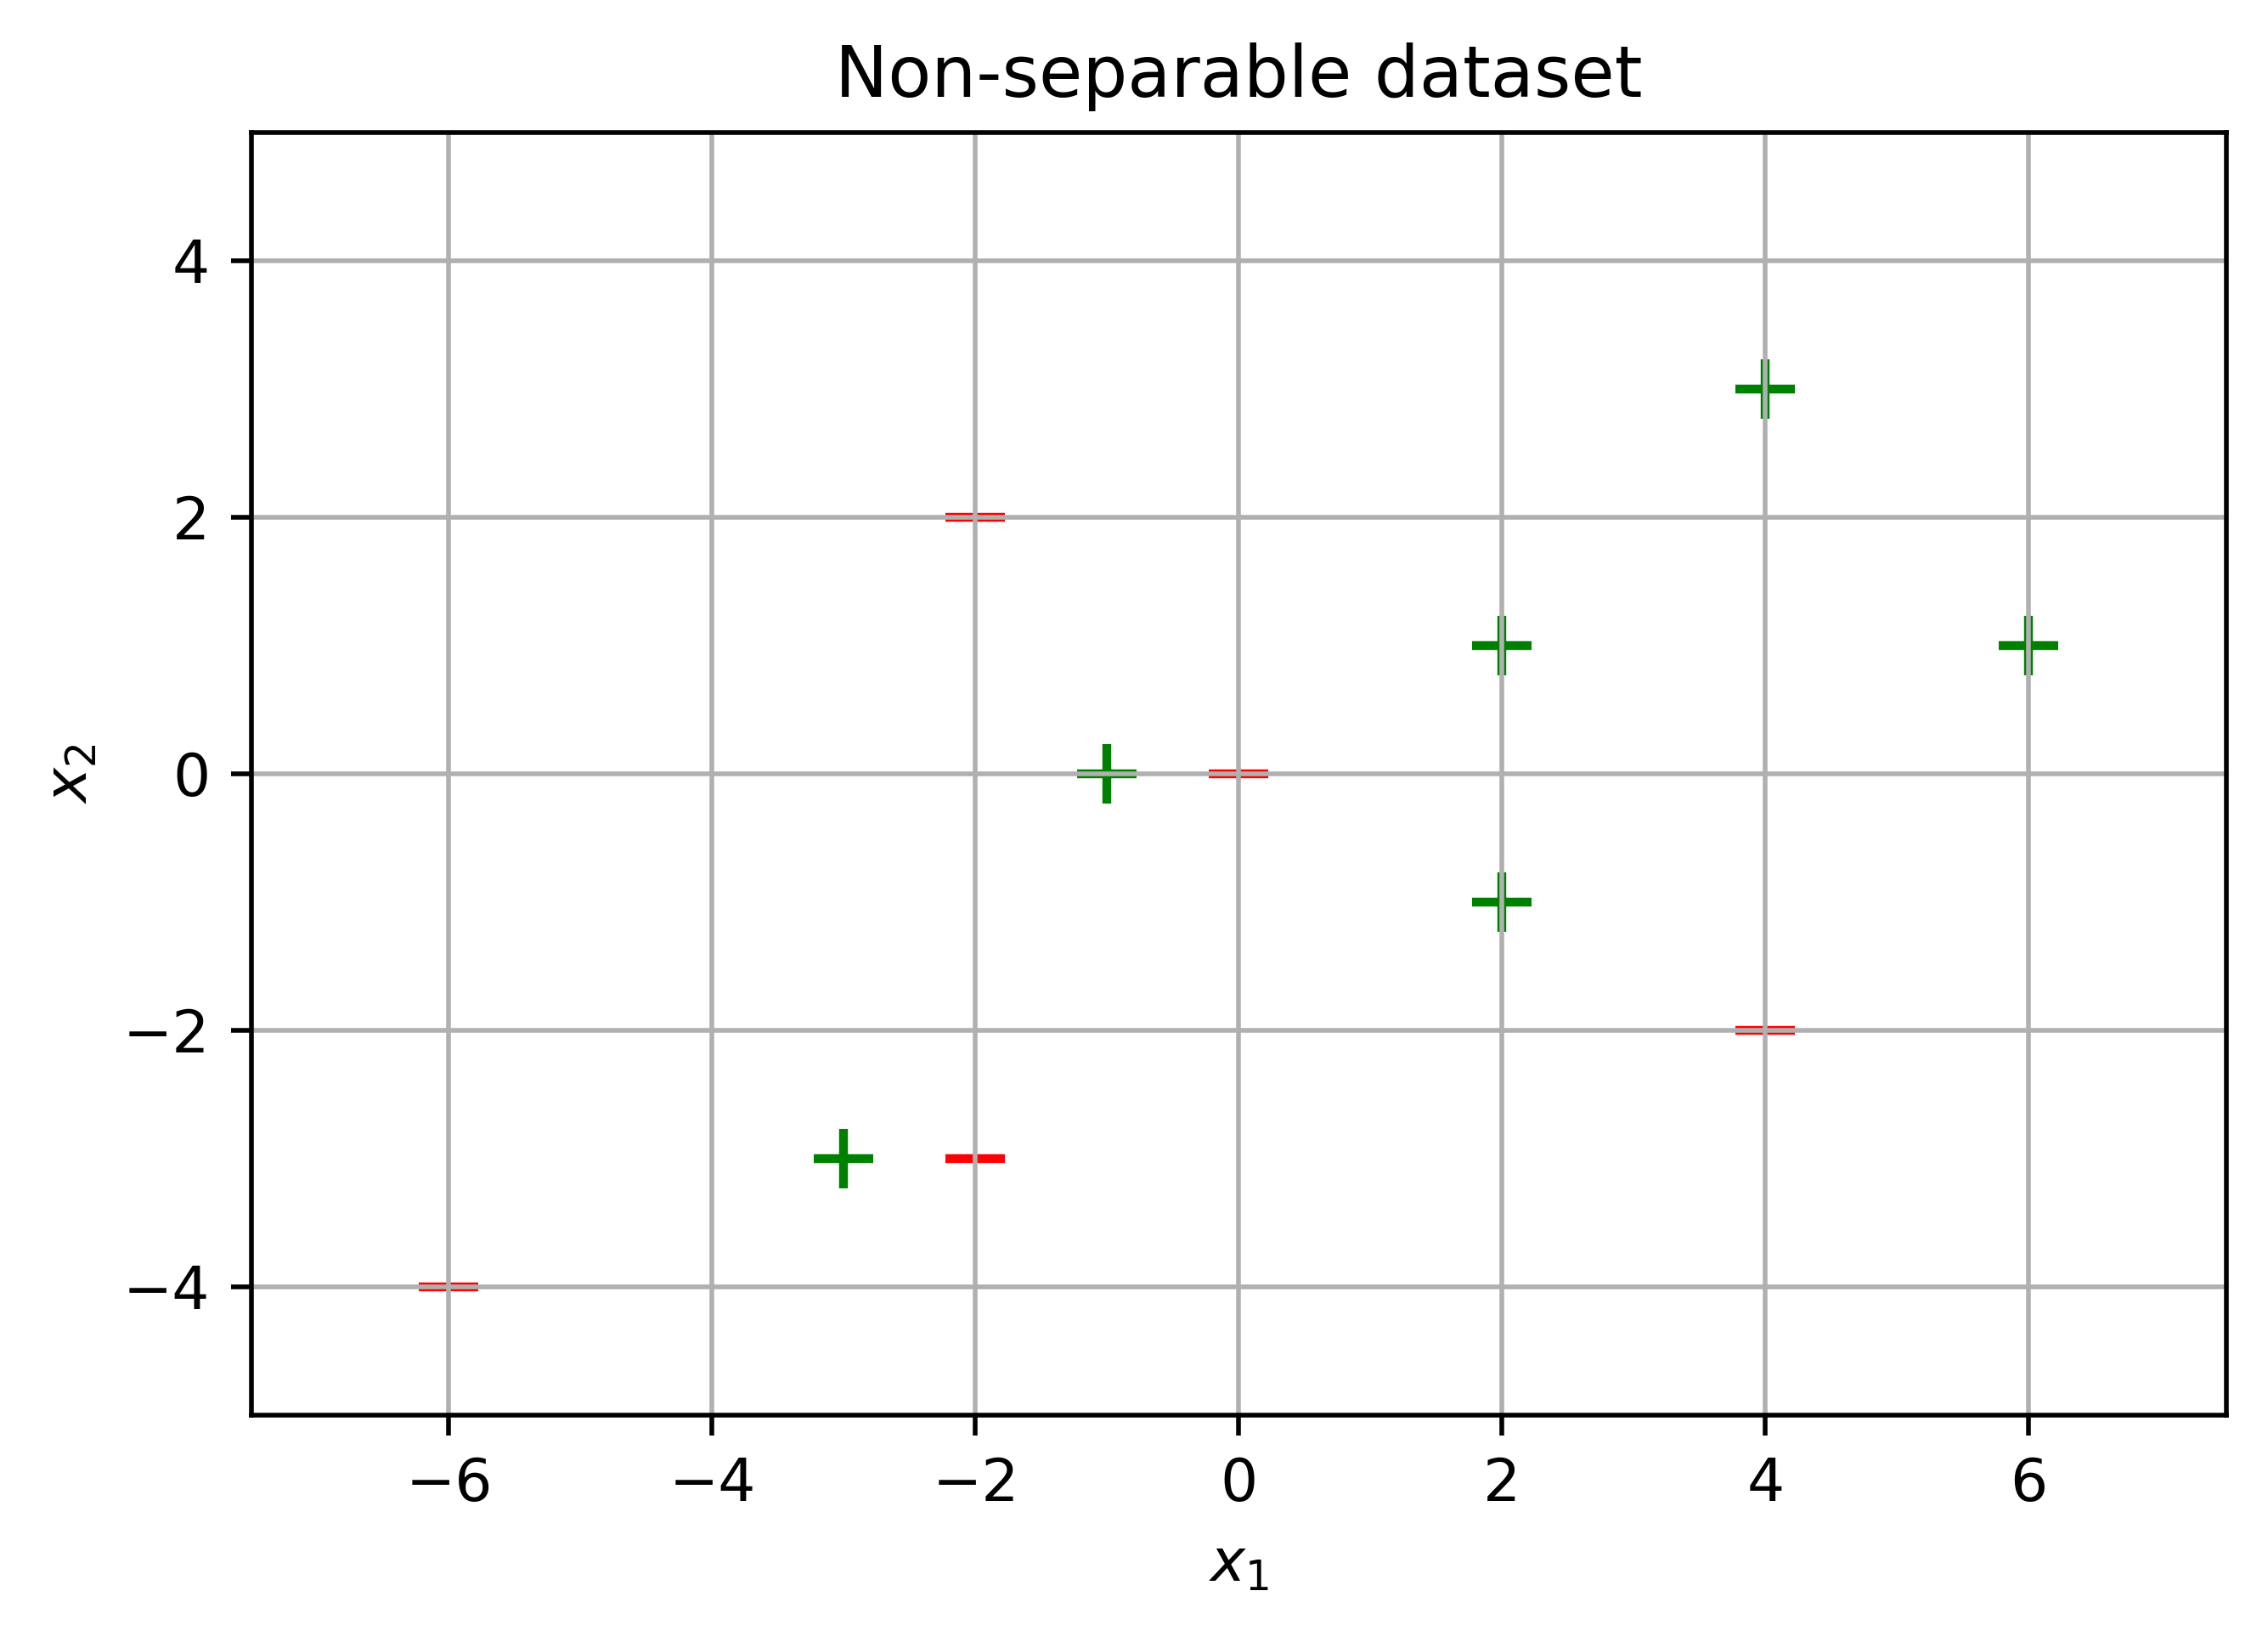
\includegraphics[width=70mm,scale=0.5]{images/classification_images/non_separable_dataset.png}
            \caption*{There's no line we could draw through this data to \textbf{separate} the points from each other.}
        \end{figure}
            
        If we can, we call it \textbf{linearly separable}.\\
        
        \begin{definition}
            A \gren{dataset} is \vocab{linearly separable} if you can \purp{perfectly} classify it with a \gren{linear classifier}.
        \end{definition}
        
        A couple common reasons for data to not be linearly separable:
        
        \begin{itemize}
            \item A positive and negative data point have the exact\textbf{ same position} in input space.
            
            \item Two points on either \textbf{side} of a point with opposite classification: $+-+$ or $-+-$, for example.
        \end{itemize}
        
        Very often, real-world datasets \textbf{can't} linearly separated, because of \textbf{complexities} in the real world, or random \textbf{noise}.
        
        But, sometimes, we can \textbf{almost} linearly separate it: we get very high \textbf{accuracy}. In those cases, it may be \textbf{fine} to use a linear separator: we might risk \textbf{overfitting} if we use a more complex model.
            \note{What is "high enough accuracy"? Depends on what you need it for!}
        
        Still, if a dataset is not \textbf{linearly separable}, or at least \textbf{high-accuracy} with a linear separator, that could mean we need a \textbf{richer} hypothesis class. 
            \note{Remember: a "richer" or more "expressive" hypothesis class is one that can create more hypotheses that our current one can't!}
        
        We'll get into ways to make a \textbf{richer} class in the \textbf{next} chapter: \textbf{feature transformations}.
